\documentclass[11pt,a4paper]{scrartcl}
\usepackage[utf8]{inputenc}
\usepackage[ngerman]{babel}
\usepackage{amsmath}
\usepackage{amsfonts}
\usepackage{amssymb}
\usepackage{makeidx}
\usepackage{hyperref}
\usepackage{colortbl}
\usepackage{listings}
\usepackage{chngcntr}
\usepackage{upgreek}
\usepackage{pgfplots}
\pgfplotsset{compat = newest}
\usepackage{amsthm}
\usepackage{ulem}
\usepackage{tikz}
\usepackage{graphicx}
\usetikzlibrary{positioning}
\usepackage{tikz-network}
\usepackage[left=3cm,right=3cm,top=3cm,bottom=3cm]{geometry}

\usepackage[backend=biber, style=alphabetic]{biblatex}
\addbibresource{literature.bib}
\author{Roman Wetenkamp}
\title{Systemnahe Programmierung}
\subtitle{Technische Informatik II}

\newtheorem{note}{Bemerkung}
\newtheorem{definition}{Definition}
\newtheorem{satz}{Satz}
\newtheorem{theorem}{Theorem}
\newtheorem{lemma}{Lemma}
\newtheorem{example}{Beispiel}

\lstset{extendedchars=\true ,inputencoding=utf8}

\newlength{\stackWidth}
\setlength{\stackWidth}{5cm}

\newlength{\smallestHeight}
\setlength{\smallestHeight}{11pt}

\tikzset{block2/.style={shape=rectangle, draw, node distance=-1pt, minimum width = \stackWidth, line width=1pt, inner sep=0pt}}

\begin{document}
\vspace{3cm}
\maketitle
\begin{center}

\includegraphics[scale=0.7]{DHBW.jpg}
\end{center}
\pagebreak
\tableofcontents
\pagebreak
\section*{Vorwort}
Liebe Mitstudierende, \\\\
Systemnah Programmieren -- Klingt komplizierter als es ist. Vielleicht habt ihr euch schon einmal einen Elektronik-Adventskalender oder -baukasten schenken lassen, um damit herumzuspielen, einen Feuchtigkeitssensor für Blumenerde zu entwickeln oder die intelligente Wäscheklammer? In diesem Modul widmen wir uns genau diesem Gebiet, dem hardwarenahen Herumtüfteln an Mikrocomputern. \\\\
In diesem Skript notieren wir alles Relevante aus der Vorlesung, ergänzen es um ein paar Aufgaben und Anmerkungen und bereiten uns so auf die Klausur vor. Dieses Skript basiert auf der Vorlesung von Joachim Wagner an der DHBW Mannheim im Studiengang Informatik -- Cyber Security, die Passgenauigkeit für andere Dozierende oder Jahrgänge kann ich nicht beurteilen. \\\\
\textit{Viel Erfolg!}  \\
\begin{flushright}
Roman Wetenkamp \\
Mannheim, den \today
\end{flushright}  
\vfill
\paragraph{Fehlerfinden}
Mein Dank gilt folgenden Personen, die Fehler gefunden, korrigiert und so dieses Skript verbessert haben: 
\begin{itemize}
\item Daniel Riebel
\item Finn Callies
\item Gurleen Kaur Saini
\end{itemize}
\paragraph{Warnung}
Das Studium an einer Dualen Hochschule unterscheidet sich von dem Studium an Universitäten oder regulären Fachhochschulen insbesondere dadurch, dass aufgrund der Dualität von Theorie und Praxis meist nur die Hälfte der Zeit zur Vermittlung des Stoffes zur Verfügung steht (wenn dann auch intensiver). Daher gehen Sie bitte nicht davon aus, dass Sie dieses Skript ausreichend auf Klausuren in regulären Vollzeitstudiengängen vorbereitet!
\paragraph{Hinweis}
Dieses Dokument ist kein Vorlesungsmaterial, hat nicht den Anspruch auf {Voll}\-{ständigkeit} und enthält mit Sicherheit Fehler. Des Weiteren ist es noch lange nicht vollendet (es ist infrage zustellen, ob es das je sein wird), und doch möchte ich Sie ermutigen, beizutragen! Jegliche Fehler, Probleme oder Anmerkungen können Sie mir gerne über das dazugehörige GitHub-Repository unter der URL \url{https://github.com/RWetenkamp/sysprog} zukommen lassen. Danke!
\pagebreak
\part{Einfache Ein-/Ausgabe-Prozesse}
\section{Einführung}
Systemnah zu programmieren bedeutet zuallererst, viele Ebenen der Abstraktion, die Betriebssysteme oder Virtualisierungen hinter sich zu lassen und zurückzukehren zu dem grundlegendsten Konzept der Computertechnik, dem Bit. \\
\begin{definition}
Ein Bit ist die kleinste Speichereinheit eines Computersystems. Der Wert eines Bits ist entweder \textbf{0} für \textbf{aus} oder \textbf{1} für \textbf{ein}. Sprechen wir von einem 8-Bit-Register, so bezeichnen wir damit acht einzeln adressierbare Werte, die jeweils auf 0 oder 1 gesetzt werden können. 
\[8 \text{ Bit } \widehat{=} 1 \text{ Byte }\]
\end{definition}

Sie werden in Ihren Programmen verschiedene Bitoperationen implementieren müssen, da die zugrundeliegende Hardware zu großen Teilen aus Registern besteht, die sie auf diese Weise ansprechen können.
\begin{table}[h]
\centering
\begin{tabular}{|l|c|c|c|c|c|}
\hline
Bezeichnung & Symbol & C-Operatorsymbol & $a$ & $b$ & Ergebnis \\
\hline
Konjunktion & $\land$ & \texttt{\&} & 0 & 0 & 0 \\
&&&0 & 1 & 0 \\
&&&1 & 0 & 0 \\
&&&1 & 1 & 1 \\
\hline
Disjunktion & $\lor$ & \texttt{|} & 0 & 0 & 0 \\
&&&0 & 1 & 1 \\
&&&1 & 0 & 1 \\
&&&1 & 1 & 1 \\
\hline
XOR & $\oplus$ & \texttt{\^} & 0 & 0 & 0 \\
&&&0 & 1 & 1 \\
&&&1 & 0 & 1 \\
&&&1 & 1 & 0 \\
\hline
\end{tabular}
\caption{Übersicht über binäre Bitoperationen}
\end{table} \\

\begin{table}[h]
\centering
\begin{tabular}{|l|c|c|c|c|c|}
\hline
Bezeichnung & Symbol & C-Operatorsymbol & $a$ & Ergebnis \\
\hline
Negation & $\lnot$ & \texttt{~} & 0 & 1 \\
&&&1 & 0 \\
\hline
Linksverschiebung & &\texttt{<<} & 0000 & \texttt{1 << 1}: 0001, \texttt{1 << n}: 00...1...0 \\
\hline
Rechtsverschiebung & & \texttt{>>} & 1000 & \texttt{1 >> 1}: 0100, \texttt{1 >> n}: 00...1...0 \\
\hline
\end{tabular}
\caption{Übersicht über unäre Bitoperationen}
\end{table}

Im folgenden Kapitel betrachten wir die verwendete Hardware und beginnen damit, die einzelnen Bestandteile und ihre Aufgaben zu erläutern. Wir werden jeweils anhand von Beispielprogrammen zeigen, wie die einzelnen Komponenten angesprochen und programmiert werden können. Die Programmiersprache hierfür ist C, in der Vorlesung wurde das {\glqq}Mikrochip Studio{\grqq} als IDE verwendet. Sie können es hier beziehen: 
\href{https://www.microchip.com/en-us/development-tools-tools-and-software/microchip-studio-for-avr-and-sam-devices}{Microchip Studio}

\section{Hardware}
Grundlegend ist Ihnen der Aufbau eines Computersystems sicherlich vertraut.
\begin{itemize}
\item Die \textbf{CPU} (Central Processing Unit), also der Prozessor, ist die zentrale Komponente, die die Befehle ausführt.
\item Während der Ausführung speichert die CPU Programmdaten im Arbeitsspeicher, dem \textbf{RAM} (Random Access Memory). Dieser Speicher wird nur zur Laufzeit genutzt und ist daher nicht persistent.
\item Ebenso gibt es einen Massenspeicher, eine Festplatte, auf der Daten persistent gespeichert werden und bei Bedarf gelesen/geschrieben werden.
\end{itemize}
Diese Grundstruktur gleicht im Wesentlichen dem \textsc{Von-Neumann-Prinzip} und ist sowohl auf klassische PCs anwendbar als auch auf Mikrocontroller, denen wir uns im Rahmen dieser Vorlesung widmen wollen.
\\
\begin{note}
Ein \textbf{Mikrocontroller} ist ein Minicomputer auf einem Chip. Er enthält einen Mikroprozessor und Speicher.
\end{note}
Ein solcher Mikrocontroller findet sich häufig auf Entwicklungsboards, wie z. B. der Arduino-Produktfamilie, die bereits aufgelötete Ports für weitere Komponenten enthalten. Derartige Boards gibt es zuhauf im Markt. Häufig sind die Unterschiede gering, da Arduino-Boards unter einer Open-Source-Lizenz stehen und somit von anderen ohne Weiteres kopiert werden dürfen. \\\\
Im Rahmen dieser Vorlesung arbeiten wir mit Arduino-Mikrocontrollern oder zu Arduino kompatiblen Äquivalenten. Die von uns verwendeten Boards enthalten allesamt folgenden Mikroprozessor:
\begin{center}
\textbf{ATMEL ATmega 328P}
\end{center}
Die Kenntnis des Mikrocontrollers ist unabdingbar für den weiteren Verlauf der Vorlesung. \\
Die Mikrocontroller Arduino Uno und Arduino Nano enthalten genannten Prozessor. Wir werden als Referenz jeweils den Arduino Uno verwenden.
\begin{figure}[h!]
\centering
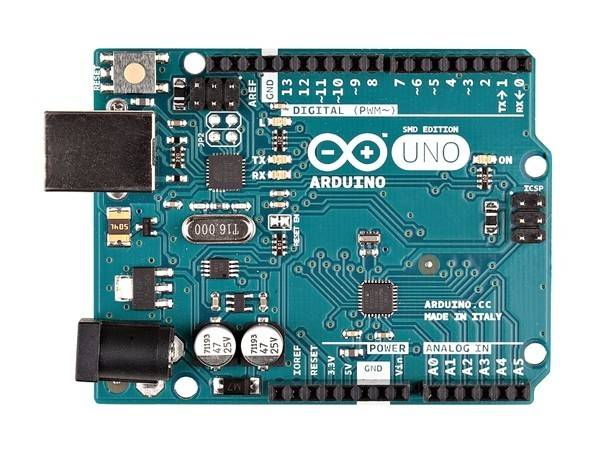
\includegraphics[scale=0.4]{uno.png}
\caption{Arduino Uno mit ATMEL ATmega328P}
\end{figure}
\paragraph{Aufbau}
Dieser Mikrocontroller enthält einige relevante Komponenten, die über einen Bus mit der CPU verbunden sind. Wir entnehmen diese dem folgenden Blockschaltbild.
\begin{figure}[h!]
\centering
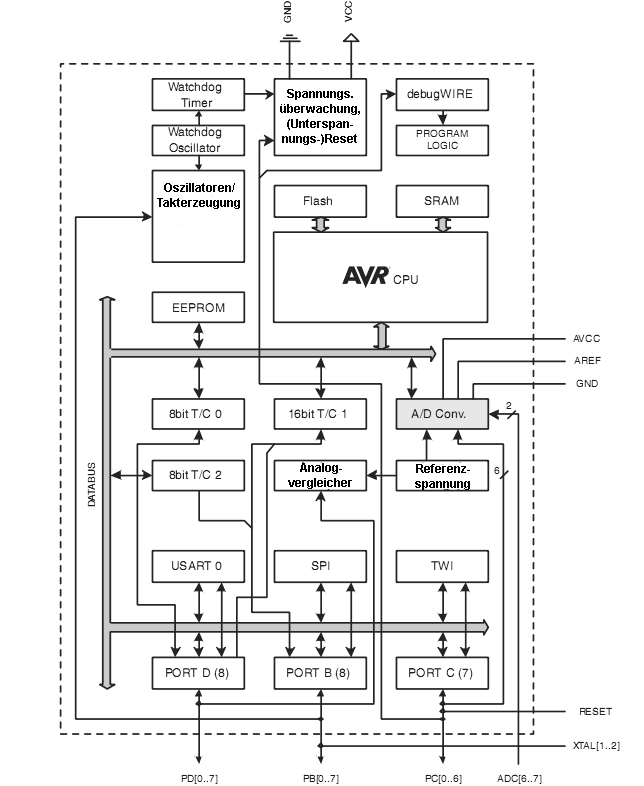
\includegraphics[scale=0.5]{b2-1.png}
\end{figure}
\begin{itemize}
\item \textbf{Flash} -- Der Flash-Speicher ist neben SRAM und EEPROM einer der drei Speichertypen. Der Flash-Speicher ist unveränderlich und kann lediglich von außen gebrannt werden. Hier wird das aktuelle Skript / Programm gespeichert.
\item \textbf{SRAM} -- Hierbei handelt es sich um einen winzig kleinen Arbeitsspeicher. Dieser Speicher ist nicht persistent und wird von der CPU während der Laufzeit verwaltet und verwendet.
\item \textbf{EEPROM} -- Dieser Speicher ist persistent und fungiert als {\glqq}Festplatte{\grqq}.
\item \textbf{Watchdog} -- Sollte der Chip nach einer gewissen Zeit kein Lebenssignal mehr senden, setzt der Watchdog den Mikrocontroller automatisch zurück.
\item \textbf{A/D Converter} -- Die Prozessoren der ATmega-Reihe können analoge Signale in digitale umwandeln. Dafür ist dieser Baustein zuständig.
\item \textbf{8/16bit T/C} -- Diese Bauteile sind Timer/Counter, die zur Prozesssteuerung genutzt werden können. Wir widmen uns diesen Bauteilen später.
\item \textbf{USART} -- Eine serielle Schnittstelle für diversen Datenverkehr ist der USART-Baustein.
\item \textbf{TWI} -- Die TWI-Schnittstelle kann für die Verknüpfung mehrerer Mikrocontroller untereinander genutzt werden.
\end{itemize}
Im Allgemeinen wird die Kommunikation mit jeder Hardware/CPU über I/O-Ports abgewickelt. 
\begin{note}
Gelegentlich kann es zu Verwirrung kommen, da sowohl internen I/O-Ports des Mikrocontrollers als auch die Anschlusspins für elektronische Bauteile als \textbf{Ports} bezeichnet werden. Im Kontext dieses Kurses bezeichnen wir letztere als {\glqq}Beinchen{\grqq}.
\end{note}
\paragraph{System} Der hier gezeigte Controller folgt der \textbf{RISC}-Architektur. RISC steht für {\glqq}Reduced Instruction Set Controller{\grqq}. Es hat sich gezeigt, dass mit einem im Vergleich zu Assembler reduzierten Befehlssatz ähnlich effizient, jedoch viel leichter dekodierbar und in der Regel schneller, gearbeitet werden kann. Der Mikrocontroller enthält von sich aus kein Betriebssystem. Wollen wir ein Programm ausführen, so müssen wir dieses speziell für diesen Mikroprozessor in einer hardwarenahen Programmiersprache wie Java oder C implementieren.
\section{Grundlegendes zur Programmierung}
Wir werden in dieser Vorlesung -- und damit auch in diesem Skript -- die Programmiersprache C verwenden. Um die benötigten Bibliotheken nutzen zu können, müssen die passenden Treiber installiert werden. Am einfachsten lässt sich dies durch die Arduino IDE und das zuvor erwähnte Microchip Studio realisieren. Das \textbf{Flashen}, also das Aufspielen der Programme auf das Board, erfolgt über USB.
\paragraph{Programmaufbau}
Wie Sie es von C gewohnt sein werden, unterscheiden wir \textbf{Programmzeilen} und \textbf{Präprozessordirektiven}. Die Befehle, die ausgeführt werden sollen, müssen Bestandteil der \texttt{main()}-Funktion des Programms sein.
\begin{note}
Jedes Programm, dass Sie flashen wollen, muss eine Endlosschleife enthalten! Andernfalls wird die Operation lediglich ein einziges Mal ausgeführt.
\end{note} 
Angewandt bedeutet dies:
\begin{lstlisting}[language=C]
#define F_CPU 16000000UL
#include <avr/io.h>

int main() {
	// Initialisierungen
	while(1) {
		// Hier koennen Sie Ihren Code platzieren	
	}
}
\end{lstlisting}
Sie erkennen die Definition der Konstante F{\_}CPU in der ersten Zeile. Hier legen wir fest, dass der Prozessor mit einem Takt von 16 MHz arbeitet.
\subsection{Register und Ports}
Unser Ziel ist es, verschiedene elektronische Bauteile an den Ports des Microcontrollers anzuschließen und mit diesem interagieren zu lassen. Dafür veranschaulichen wir uns zunächst die Pinbelegung des Boardes.
\begin{figure}[h!]
\centering
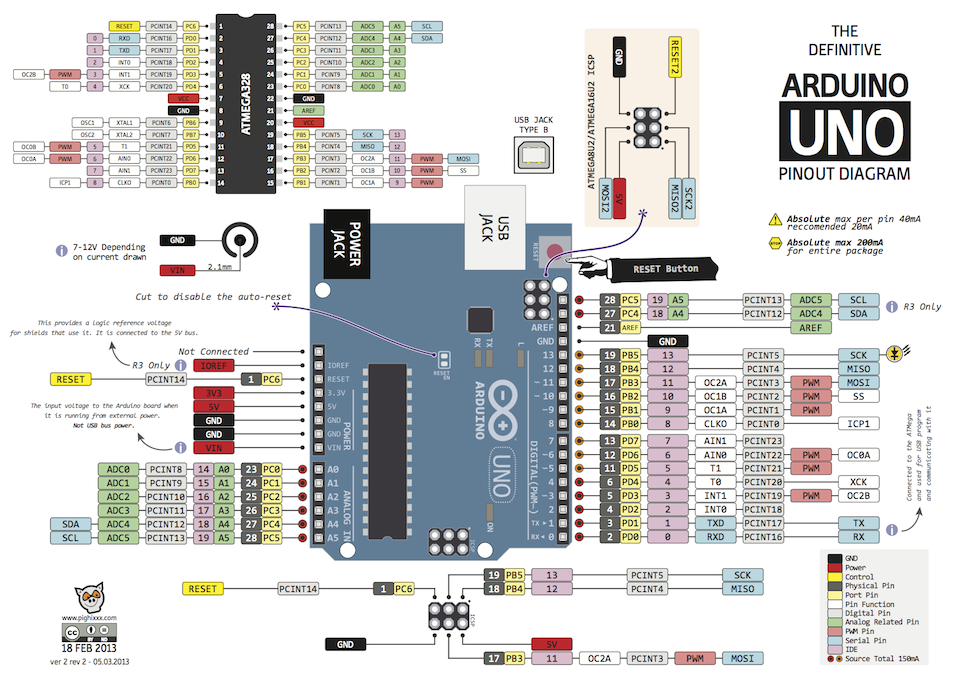
\includegraphics[scale=0.8]{pins.png}\label{pins}
\caption{Pinbelegungen des Arduino Unos}
\end{figure}
Von Relevanz für das nun folgende programmatische Ansprechen der Pins sind die hier gelb hinterlegten {\glqq}Port Pin{\grqq}-Belegungen, also beispielsweise der Port \textbf{PB5} an Pin 19 bzw. Onboard-IDE 13. Wir erkennen, dass es drei mal acht dieser Ports gibt, die Register PB (für Port B), PC und PD. Diese Ports nutzen wir -- wie angesprochen -- um zusätzliche Bauteile anzusprechen. \\\\
Für jeden dieser 24 Pins müssen wir festlegen, ob es sich um eine Input- oder Output-Port handelt. Diese Informationen halten wir im \textbf{DDR (Data direction register)} fest.
\paragraph{Programmzeilen} \quad
\begin{lstlisting}[language=C]
DDRB |= (1 << DDB5);					// (1)

DDRD |= (1 << DDD3) | (1 << DDD4) | (1 << DDD5);	// (2)

DDRD &= ~(1 << DDD2);					// (3)
\end{lstlisting}
\begin{itemize}
\item[(1)] Im Data Direction Register B verschieben wir eine 1 an die Stelle des fünften Bits, um Pin B5 als Ausgang zu definieren. Wir verwenden die Disjunktion, um andere, möglicherweise bestehende Eingaben, nicht zu überschreiben. Alternativ dazu ließe sich das Register selbstredend auch durch eine Angebe der Art \texttt{0b00100000} initialisieren, falls man beabsichtigt, nur das Bit 5 als Ausgang zu definieren.
\item[(2)] In dieser Zeile gehen wir ähnlich vor und initialisieren das DDR D. Nun soll jedoch nicht bloß ein einzelnes Bit initialisiert, sondern drei gleichzeitig, die wir gegenseitig disjunktiv verknüpfen.
\item[(3)] Nun bleibt noch, einen Pin wie hier als Eingang zu definieren. Da sich Nullen binär nicht schieben lassen, arbeiten wir hier mit der Negation der 1-Shift-Operation.
\end{itemize}
Im nächsten Kapitel betrachten wir die Möglichkeiten des Einlesens genauer, insbesondere behandeln wir dort Interrupts. \\\\
Mit der Definition des DDRs für die entsprechenden Bits ist die Hälfte getan. Wollen wir nun die Systemspannung von 5 V an einen spezifizierten Port anlegen, gehen wir analog vor:
\begin{lstlisting}[language=C]
PORTB |= (1 << PORTB5);			// einschalten
PORTB &= ~(1 << PORTB5);		// ausschalten
\end{lstlisting}
\subsection{Eingangssignale}
In vielen Schaltungen verwenden wir Taster und Schalter, um auf Benutzereingaben zu reagieren. Diese Bauelemente beeinflussen die Ströme, in dem eine Spannung erst bei Tastendruck anliegt oder dann nicht mehr. Der Microcontroller liest diese Spannungen nun aus und interpretiert sie entsprechend mit 0/1 (an/aus). Für dieses Verfahren gibt es zwei Varianten:
\begin{itemize}
\item \textbf{Polling} -- Hierbei wertet das Programm intervallbasiert die anliegende Spannung am Pin des Bauelements aus. Dieses Vorgehen ist ressourcenintensiv und daher nach Möglichkeit zu vermeiden.
\item \textbf{Interrupts} -- Effizienter hingegen ist es, wenn das Programm durch einen vordefinierten Interrupt unterbrochen wird. Dieses Verfahren wird im nächsten Kapitel ausführlicher behandelt.
\end{itemize}
Eine allgemeine Schwierigkeit beim Einlesen der Daten liegt aufgrund des \textbf{Prellens} vor. So verläuft der Spannungswechsel zwischen 0 und 5 V längst nicht so sauber, wie es wünschenswert ist. Stattdessen kann es bis zu 10 Sekunden dauern, bis ein klares Signal vorliegt,
 da elektromagnetische Spannungen und Wellen die gemessene Spannung verändern. Um diesem Phänomen zu begegnen, werden sogenannte \textbf{Pull-Up-Widerstände} eingesetzt, die dafür sorgen, dass die Spannung im nicht gedrückten Zustand {\glqq}hochgehoben{\grqq} wird und im Falle des Tastendrucks spürbar abfällt. Der Widerstand hat hierbei häufig den Wert $4.7 \text{ k}\Omega$.
\begin{figure}[h!]
\centering
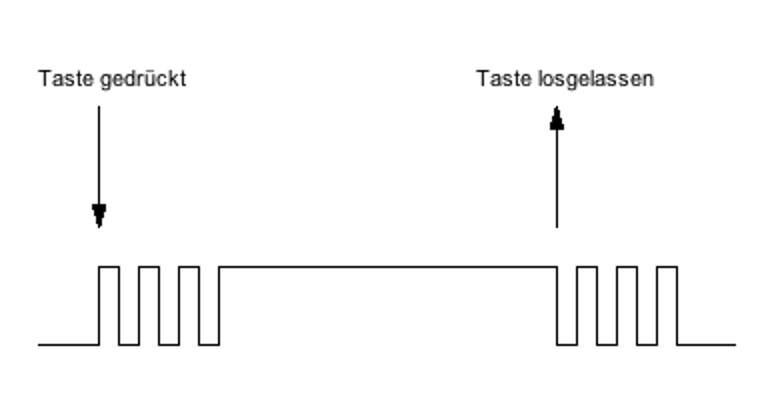
\includegraphics[scale=0.6]{prellen.png}
\caption{Prellen eines Tasters}
\end{figure}
\section{Programmbeispiele}
An dieser Stelle will ich die relevantesten Programme aus der Vorlesung abbilden, um sie reproduzierbar zu machen.
\subsection{Blinken}
Ein Standard-Beispiel, um zu testen, ob ein Arduino-Board funktionsfähig ist, ist das \textbf{Blink}-Beispiel. Wir wollen die Onboard-LED des Boards in einem vordefinierten Intervall zum Blinken bringen.
\paragraph{Schaltung} Für dieses Beispiel müssen keine weiteren Komponenten an das Board angeschlossen werden. Wir verwenden lediglich die bereits fest verlötete Onboard-LED.
\paragraph{Programm} \quad
\begin{lstlisting}[language=C]
/*
 * Blinken
 *	
 */ 

#define F_CPU 16000000UL	// Prozessortaktkonstante
#include <avr/io.h>		// Systembibliothek
#include <util/delay.h>		// Systembibliothek

int main(void)
{
	DDRB |= (1 << DDB5);		// initialisiert B5 als Ausgangspin
	PORTB |= (1 << PORTB5);		// legt Spannung an Port B5 an
	
	while (1) 
	{
		PORTB &= ~(1 << PORTB5);	// entzieht B5 die Spannung
		_delay_ms(500);			// Wartet 500 Millisekunden
		PORTB |= (1 << PORTB5);		// setzt B5 unter Spannung
		_delay_ms(500);
	}
}
\end{lstlisting}
\subsection{Tastendruck auslesen}
Nun wollen wir zwei Taster mittels Polling auslesen und bei die Onboard-LED bei Tastendruck ein- bzw. ausschalten.
\paragraph{Schaltung} Zusätzlich zum Entwicklungsboard benötigen wir nun zwei Taster, den wir auf einem Steckbrett befestigen und mit Port D2 und D3 des Boards verbinden. Der zweite Anschluss der Taster wird mit GND (Masse) verbunden. Bezogen auf obige Grafik handelt es sich dabei um die Pins 16, 17 und 20 (GND).
\paragraph{Programm} \quad
\begin{lstlisting}[language=C]
#include <avr/io.h>

int main(void)
{
	DDRD &= ~(1 << DDD2);	// D2 ist Eingabe
	DDRD &= ~(1 << DDD3);	// D3 ist Eingabe
	
	// Pull up
	PORTD |= (1 << DDD2) | (1 << DDD3);
	
	DDRB |= (1 << PORTB5);		// Onboard-LED ist Ausgabe
	PORTB &= ~(1 << PORTB5);	// Onboard-LED ist initial aus
	
    while (1) 
    {
    		// Auslesen der Taster
		if(! (PIND & (1 << DDD2))){
			// Einschalten der LED			
			PORTB |= (1 << PORTB5);
		}
		
		if(! (PIND & (1 << DDD3))){
			// Ausschalten der LED			
			PORTB &= ~(1 << PORTB5);
		}
    }
}

\end{lstlisting}
\section*{Aufgaben}
\begin{enumerate}
\item Nennen Sie die drei unterschiedlichen Arten von Speicher. Erläutern Sie die Unterschiede.
\item Erläutern Sie das Vorgehen, um eine weitere LED vom Board aus unter Spannung zu setzen.
\item Schließen Sie eine LED an Port B3 und einen Taster an Port D2 an. Entwickeln Sie ein Programm, das beim Druck des Tasters zwischen der Onboard-LED und der externen LED umschaltet.
\end{enumerate}
\part{Interrupts}
\section{Interrupts}
Die zweite Variante, um mit Eingaben umzugehen, sind Interrupts. \\
\begin{definition}
Unter einem Interrupt verstehen wir eine kurzfristige und unmittelbare Unterbrechung der Programmausführung, um einen kurzen, zeitlich kritischen Vorgang abzuarbeiten.
\end{definition}
\paragraph{Motivation}
Dem Kontext von Eingaben nähern wir uns durch folgende Betrachtungsweise:
Während wir beim Polling fortwährend überprüfen, ob eine Bedingung eingetreten ist -- wie z. B. ein Tastendruck -- und dann auf dieses Ereignis reagieren, operieren wir bei Interrupts anders. Wir melden an, dass wir bei einem bestimmten Ereignis unterbrochen werden wollen. Tritt dieses Ereignis nun ein, wird unsere Programmausführung unterbrochen und die Behandlung des Ereignisses wird ausgeführt. Auf diese Weise besteht keine Notwendigkeit mehr, ressourcenintensiv die Bedingung fortwährend zu überprüfen, sondern viel mehr ergeben sich Möglichkeiten der Nebenläufigkeit. 
\paragraph{Umsetzung}
Wenn wir erneut die Abbildung \ref{pins} betrachten, so finden wir dort den Ports PD2 und PD3 die Bezeichnungen \textbf{INT0} und \textbf{INT1}. Diese Pins sind die einzigen direkt geschalteten Interrupt-Ports. Eine Änderung der Spannung an diesen Pins triggert die Interrupt-Routinen, die wir im Folgenden implementieren werden. Neben diesen beiden Interrupt-Pins gibt es eine Zahl weiterer, die über ein Multiplexing-Verfahren adressiert werden können. Dies war jedoch nicht Teil der Vorlesung und wird daher an dieser Stelle ausgespart. 
\paragraph{Interrupttabelle}
Für jeden möglichen Interrupt muss zentral gespeichert sein, was nach Eintritt des selbigen abläuft. Dazu steht am Anfang des Flash-Speichers die \textbf{Interrupttabelle}. So befindet sich beispielsweise für den Interrupt INT0 ein Eintrag in der Tabelle, der einen Sprungbefehl der Form \texttt{JMP 1000} oder \texttt{RETI} beinhaltet. Letzteres steht für {\glqq}Return from Interrupt{\grqq} und referenziert die Rücksprungadresse zurück in das Hauptprogramm.
\paragraph{ISR (Interrupt Service Routine)} Wir implementieren in unserem Programm sogenannte ISRs, in denen der Code steht, den wir im Falle eines Interrupts an einem spezifizierten Pin ausführen. 
\begin{lstlisting}[language=C]
ISR (INT0_vect) {
	// Programmzeilen
}
\end{lstlisting}
Der Code in den ISRs sollte so klein wie möglich sein, da die Abarbeitung per se kritisch ist und keine Interrupts ineinander ausgelöst werden sollten. Daraus folgt auch, dass keine teuren Operationen in ISRs zu erfolgen haben.
\paragraph{Konfiguration}
Um Interrupts im Programm nutzen zu können und auf Eingaben zu reagieren, müssen wir -- auf gewohnte Art und Weise -- wieder bestimmte Registereinträge ändern.
\begin{itemize}
\item \textbf{EICRA} (External Interrupt Control Register A) -- Die Bits in diesem Register spezifizieren genauer, welche Änderungen der Spannung am Interrupt-Pin die ISR auslösen. Die genauen Einstellungen hierfür sind den Datenblättern der Microcontroller zu entnehmen. Möglich ist beispielsweise, dass nur bei steigenden bzw. fallenden Flanken reagiert wird oder generell bei jedem Pegelwechsel. 
\begin{table}[h!]
\centering
\begin{tabular}{|p{1cm}|p{1cm}|p{1cm}|p{1cm}|p{1cm}|p{1cm}|p{1cm}|p{1cm}|}
\hline
7 & 6 & 5 & 4 & 3 & 2 & 1 & 0 \\
\hline
-- & -- & -- & -- & ISC11 & ISC10 & ISC01 & ISC00 \\
\hline
\end{tabular}
\caption{EICRA}
\end{table}
Dabei spezifizieren ISC11 und ISC10 zusammen INT1 und ISC01 und ISC00 INT0.
\item \textbf{EIMSK} (External Interrupt Mask Register) -- In diesem Register werden die Interrupts {\glqq}scharf geschaltet{\grqq}. Nur wenn das Bit für INT0 hier auf 1 gesetzt wurde, reagiert das Programm tatsächlich auf einen Interrupt an Pin 1.
\begin{table}[h!]
\centering
\begin{tabular}{|p{1cm}|p{1cm}|p{1cm}|p{1cm}|p{1cm}|p{1cm}|p{1cm}|p{1cm}|}
\hline
7 & 6 & 5 & 4 & 3 & 2 & 1 & 0 \\
\hline
-- & -- & -- & -- & -- & -- & INT1 & INT0 \\
\hline
\end{tabular}
\caption{EIMSK}
\end{table}
\end{itemize}
\section{Programmbeispiel}
\subsection{Lichtschalter}
Wir wollen Interrupts nutzen, um die Onboard-LED des Entwicklungsboards über zwei Schalter ein- und auszuschalten.
\paragraph{Schaltung}
Wir benötigen erneut zwei Schalter, die wir auf einem Entwicklungsboard platzieren. Jeweils einen Kontakt der Schalter verbinden wir mit GND und einen der anderen mit INT0/INT1, also PD2 und PD3.
\paragraph{Programm}\quad
\begin{lstlisting}[language=C]
#include <avr/io.h>
#include <avr/interrupt.h>	// Systembibliothek

ISR (INT0_vect) {	// ISR fuer INT0
	PORTB = 0x00;	// Schaltet die Ports an B aus
}			

ISR (INT1_vect) {	// ISR fuer INT1
	PORTB = 0xff;	// Schaltet die Ports an B ein
}


int main(void)
{
	DDRB = 0xFF;		// Alle B-Ports werden Ausgaenge
	PORTB = 0xFF;		// Schaltet alle B-Ports ein 
	
	DDRD &= ~(1 << DDD2); 	// D2 wird Eingang
	PORTD |= (1 << PORTD2);	// An D2 wird Spannung angelegt
	DDRD &= ~(1 << DDD3);	// D3 wird Eingang
	PORTD |= (1 << PORTD3);	// An D3 wird Spannung angelegt
	
	EICRA |= (1 << ISC00);	// INT0 triggert bei Pegelwechsel
	EICRA |= (1 << ISC11);	// INT1 triggert bei Pegelwechsel
	EIMSK |= (1 << INT0);	// INT0 wird scharf
	EIMSK |= (1 << INT1);	// INT1 wird scharf
	
	sei();			// set enable interrupt
	
    while (1) 
    {
    }
}
\end{lstlisting}
\section*{Aufgaben}
\begin{enumerate}
\item Erläutern Sie, inwiefern der Einsatz von Interrupts gegenüber Polling vorteilsbehaftet ist.
\item Nennen Sie Anforderungen an ISRs.
\item Bauen Sie eine Schaltung mit zwei Tastern an INT0 und INT1 und einem Summer an einem Port aus B nach Wahl auf. Entwickeln Sie ein Programm, dass die Frequenz des Summers bei Tastendruck verdoppelt (starten Sie mit einer niedrigen Frequenz) und dem Summer sofort die Spannung entzieht, sollte der andere Taster gedrückt werden (ein Not-Aus-Schalter). Verwenden Sie dafür Interrupts.
\end{enumerate}
\pagebreak
\part{Timer / Counter}
\section{Timer und Counter}
Das nächste Konstrukt, dem wir uns wimden wollen, sind Timer. Im Blockschaltbild haben wir bereits die zwei 8-Bit- und den einen 16-Bit-Timer entdeckt und nun wollen wir mit diesen arbeiten und die Theorie dahinter verstehen.
\paragraph{Allgemeine Funktionsweise}
Ein Timer ermöglicht es uns, Aussagen zur Zeit, insbesondere der Laufzeit, zu treffen und in Abhängigkeit dazu Aktionen zu realisieren. Allgemein orientiert sich das Zählen immer am Prozessortakt. Über die verschiedenen Modi, die wir später noch genauer kennenlernen werden, lässt sich jedoch z. B. festlegen, dass nur jeder achte Prozessortakt gezählt werden soll. Läuft der Zähler über, beginnt er anschließend wieder bei 0.
\paragraph{Normal- und CTC-Mode}
In welchem Modus ein Timer operiert, wird in Registern festgehalten. Für jeden Timer gibt es drei \textbf{Timer/Counter Control Register (TCCRnA, TCCRnB, TCCRnC)}.
\begin{figure}[h!]
\centering
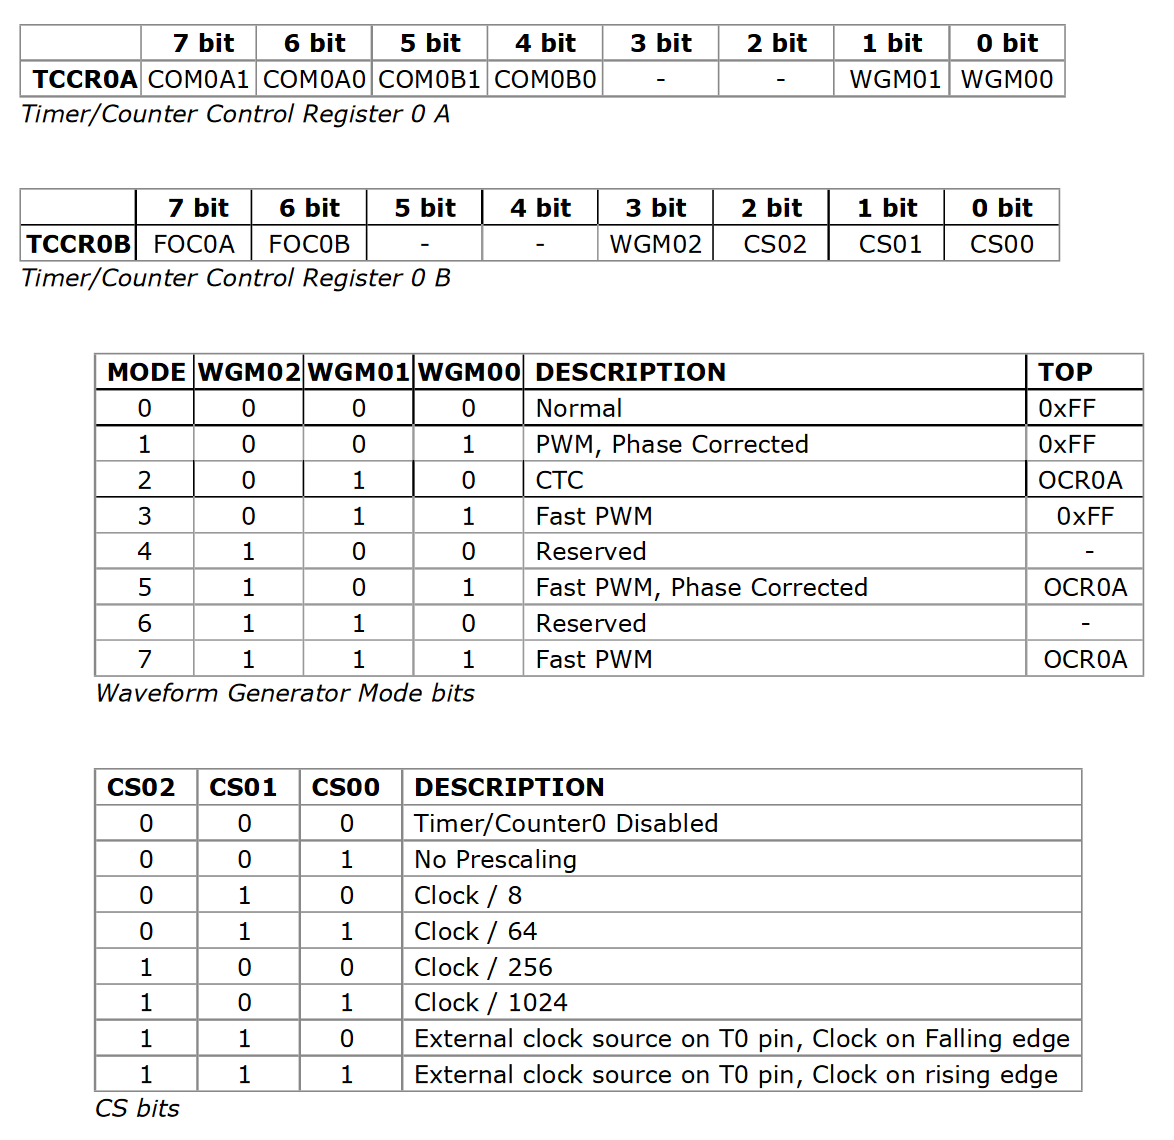
\includegraphics[scale=0.6]{timer_counter.png}
\caption{Registerübersicht}
\end{figure}
Betrachten wir nun die verschiedenen Modi (mittlere Tabelle).
\begin{itemize}
\item \textbf{Normal-Mode} -- In diesem Modus zählt der Timer die Prozessortakte bis 0xFF, also 255. Anschließend wird er zurückgesetzt und beginnt wieder bei 0. Dieser Modus wird selten eingesetzt.
\item \textbf{CTC-Mode (Clear Timer on Compare Match)} -- Ist man hingegen daran interessiert, weniger weit als 255 zu zählen, lässt sich in diesem Modus eine Zahl definieren (OCR0A), bis der gezählt wird und ab der der Counter wieder zurückgesetzt wird. Dieser Modus ist verbreiteter als der Normalmode.
\end{itemize}
Zusätzlich gibt es für beide Modi die Möglichkeit, einen Prescaler einzusetzen. Jener, ebenfalls in Registern festgelegte, Wert teilt die Frequenz des Prozessortaktes und bewirkt folglich, dass der Timer gewisse Takte ignoriert und entsprechend länger zählt. Dafür setzen wir der unteren Tabelle entsprechend die CSn-Bits. \\\\
Nun bleibt noch die Frage, wie wir auf die Ergebnisse/Werte des Timers reagieren. Für Timer im Normal- oder CTC-Mode verwenden wir hierfür Interrupts und deklarieren entsprechende ISR-Routinen. Dafür gehen wir vor wie im vorherigen Kapitel und setzen nun statt des EIMSK-Register das \textbf{TIMSKn}-Register. 
\begin{lstlisting}[language=C]
ISR (TIMER0_COMPA_vect) {
	// code
}
\end{lstlisting}
\section{PWM (Pulsweiten-Modulation)}
Weitere, signifikant andere Modi für Timer/Counter sind die der Pulsweiten-Modulation. Häufiges Einsatzfeld hierfür ist das Dimmen von LEDs. \footnote{Basierend auf \href{www.allaboutcircuits.com}{https://www.allaboutcircuits.com/technical-articles/introduction-to-microcontroller-timers-pwm-timers/}}
\paragraph{Funktionsweise von PWM im Allgemeinen} Stellen wir uns eine LED vor. Schließen wir sie ohne Timer/Counter an die Spannungsversorgung unseres Arduinos an, leuchtet sie konstant in der vorgesehenen und über den Vorwiderstand gesteuerten Helligkeit. Wir können nun einen Schalter einsetzen, der die LED alle halbe Sekunde ein- und wieder ausschaltet. Dann blinkt sie. Wenn wir nun nicht mehr von Sekunden reden, sondern sehr viel schneller ein- und wieder ausschalten, wirkt die LED dunkler und unser menschliches Auge erkennt das Schalten nicht mehr. Das nutzen wir aus. Wenn wir eine LED also nun dimmen wollen, beeinflussen wir folglich, wie groß die Intervalle zwischen Ein- und Ausschalten sind.
\begin{figure}[h!]
\centering
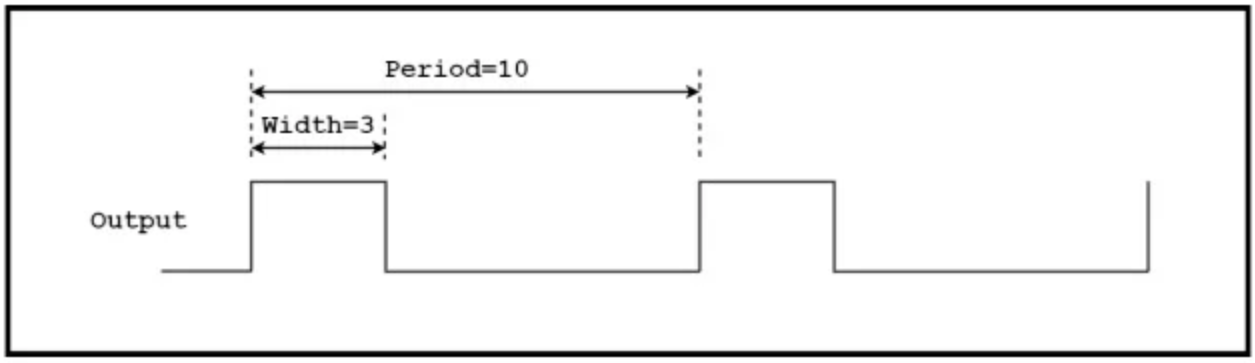
\includegraphics[scale=0.7]{pwm.png}
\caption{Darstellung von Fast PWM}
\end{figure}
Diese Technik ist besagte Pulsweitenmodulation. In der obigen Grafik wird die LED mit einer Pulsweite von 3 in einer Periode von 10 mit Spannung versorgt. Das entspricht einem \textbf{Duty-Cycle} von 30 \%. Beträgt die Breite in diesem Beispiel 5, ergäbe sich ein Duty-Cycle von 50 \%. Die Angabe erfolgt üblicherweise in Prozent.
\paragraph{Timer im PWM-Modus} Nun sind wir aber selbstredend noch daran interessiert, zu erfahren, wie denn nun Timer auf dieser Technik aufbauen. Für PWM gibt es verschiedene Modi (siehe Tabelle), in denen auch wieder festgelegt ist, ob bis 255 oder dem OCR0-Wert (Top-Wert) gezählt wird. Dieser Wert stellt die \textbf{Periode} dar. Im einfachsten Fall, dem Modus Fast PWM, funktioniert die Technik so: Zu dem Zeitpunkt, wo der Timer den Top-Wert erreicht, werden die Ausgabe-Pins der PWM-Timer unter Spannung gesetzt. Die Spannungsversorgung endet, wenn der Wert für die Pulsweite, der durch die Registerwerte für OCRA (im Fall Top=255) und OCRB (im Fall Top=OCRA) definiert ist, erreicht wird. Dann zählt der Timer bis zum Ende der Periode weiter. \\\\
Wie angedeutet, existieren zwei PWM-Modi mit leichten Unterschieden:
\begin{itemize}
\item \textbf{Fast PWM} -- Der Timer zählt von 0 bis z. B. 255, setzt nun die Pins unter Spannung, bis Compare Match eingetreten ist (OCRA-Wert). Nun wird weitergezählt, bis erneut 255 erreicht ist.
\item \textbf{Phase-corrected PWM} -- Der Timer zählt von 0 bis z. B. 255 und entzieht den Pins auf dem {\glqq}Hinweg{\grqq} die Spannung, wenn der entsprechende Wert erreicht wurde. Ist TOP (also 255) erreicht, wird nicht wieder bei 0 begonnen, sondern es wird jetzt rückwärts gezählt und beim Vergleichswert werden die Pins wieder mit Spannung versorgt. So ergibt sich eine symmetrischere Spannungskurve. 
\end{itemize}
\paragraph{Signalausgabe} In bekanntem Schaltbild \ref{pins} können wir eine Reihe an Pins entnehmen, die mit dem Zusatz \textbf{PWM} gekennzeichnet sind. Diese Pins sind in der Lage, ein PWM-Signal auszugeben. Für den ersten Timer, den wir nutzen, ist dies beispielsweise an Pin D6 der Fall.
\section{Programmbeispiel}
\subsection{LED dimmen über PWM-Timer}
\paragraph{Schaltung}
Wir schließen die Anode einer LED mit Vorwiderstand an den Port D6 und die Kathode an GND an. Der passende Vorwiderstand ist abhängig von der Spezifikation der LED.
\paragraph{Programm} \quad
\begin{lstlisting}[language=C]
#define F_CPU 16000000UL
#include <avr/io.h>
#include <util/delay.h>

int main(void)
{
	DDRD |= (1 << DDD6);
	PORTD |= (1 << PORTD6);
	
	OCR0A = 0;
	
	// Counter is now non-inverting
	TCCR0A |= (1 << COM0A1);
	
	// Set counter in PWM mode (fast PWM)
	TCCR0A |= (1 << WGM02) | (1 << WGM01) | (1 << WGM00);
	
	// Set prescaler = 8
	TCCR0B |= (1 << CS01);
    
    while (1) 
    {
		while (1) {
			// Increment OCR0A and wait 25 ms
			OCR0A += 1;
			_delay_ms(25);
		}
	}
}
\end{lstlisting}
\section*{Aufgaben}
\begin{enumerate}
\item Erläutern Sie die Möglichkeiten, auf Timer-Ereignisse programmatisch zu reagieren. Gehen Sie dabei auf die unterschiedlichen Modi ein.
\item Berechnen Sie die OCRA-Werte für folgende Duty-Cycles und TOP-Werte und erläutern Sie die Bedeutung der einzelnen Werte.
\begin{itemize}
\item 45 \% Duty-Cycle bei einem TOP-Wert von 0xFF
\item 70 \% Duty-Cycle bei einem TOP-Wert von 128
\item 10 \% Duty-Cycle bei einem TOP-Wert von 64
\end{itemize}
\item Erweitern Sie das dargestellte Programm so, dass nun zwei LEDs invers zueinander hoch- bzw. heruntergedimmt werden. Die eine LED soll folglich genau dann am stärksten leuchten, wenn die andere nicht leuchtet. Begründen Sie Ihre Ansätze.
\end{enumerate}
\pagebreak
\part{Serielle Schnittstellen}
In diesem Kapitel wollen wir uns kurz und bündig mit seriellen Schnittstellen beschäftigen. Serielle Schnittstellen nutzen wir, um zwischen Geräten auf einfache und kostengünstige Weise zu kommunizieren. Eine bekannte serielle Schnittstelle, die nicht mehr aus unserem Alltag wegzudenken ist, ist USB (Universal Serial Bus). \\
Auch Entwicklungsboards haben serielle Schnittstellen:
\begin{itemize}
\item \textbf{USART}
\item \textbf{USB}
\end{itemize}
Auf unserem Arduino-Board finden wir die Bezeichnungen {\glqq}RX{\grqq} und {\glqq}TX{\grqq} an den Ports 0 bzw. 1. Dabei steht RX für Receiver und TX für Transmitter. Halten wir also fest: Die serielle Übertragung erfolgt über mindestens zwei Leiter und ist duplex. In der Praxis wird neben beiden Leitern ein zusätzlicher Masse-Leiter verwendet.
\paragraph{Art der Übertragung}
Bei der seriellen Übertragung gibt die Pulsweite an, ob eine 0 oder eine 1 versendet und empfangen wird. Den Start und das Ende der Kommunikation wird durch Start- und Stop-Bits indiziert.
\begin{figure}[h!]
\centering
\includegraphics[scale=0.8]{Serial.png}
\caption{Beispielhafte Serielle Kommunikation}
\end{figure}
Ein Start-Bit wird durch den Abfall der Spannung gekennzeichnet, ein Stop-Bit durch den Wiederanstieg und das konstante Halten der Spannung auf 5 V. \\\\
Die Übertragungsgeschwindigkeit wird durch die \textbf{Baudrate} angegeben. Wichtig ist, dass diese Rate auf beiden teilnehmenden Geräten gleich konfiguriert ist. Ein typischer Wert ist 9600. Desto kleiner die Rate gewählt wird, desto sicherer ist die Übertragung. Für den ATmega328P stellen wir die Rate über die Register \textbf{UBRR0H} und \textbf{UBBR0L} ein.
\\
\begin{note}
Auf die Angabe eines Beispielprogramms wird aus Zeitgründen und aufgrund einer vermutlich verringerten Klausurrelevanz verzichtet. Falls Sie ein Beispielprogramm entwickelt haben, können Sie es gerne an dieser Stelle einfügen! Danke!
\end{note}
\pagebreak
\part{Programmieren in C}
\begin{flushright}
{\glqq}Aber hatten wir da nicht schon eine Vorlesung im ersten Semester zu?{\grqq}
\end{flushright}
Ja, die hatten wir. Ich denke, ich spreche nicht nur für mich, wenn ich sage, dass davon entweder vieles wieder weggenebelt ist oder auf sonderbare andere Weise nicht den Eingang in unsere Köpfe gefunden hat. Also gehen wir an dieser Stelle auf einige, relevante Charakteristika der Programmiersprache ein.
\section{Modularisierung}
Ein durchaus relevantes Prinzip der modernen Programmierung ist jenes der Wiederverwertbarkeit und Modularisierung. Wir lagern Funktionen, die wir häufiger aufrufen, die in sich abgeschlossen sind oder die für andere Projekte relevant sein könnten, in Modulen aus. 
\subsection{Verwendung nicht definierter Funktionen} 
Wenn wir in C eine Funktion aufrufen, die bis dato weder definiert noch mit einem Funktionsprototypen {\glqq}vorangekündigt{\grqq} wurde, legt C ein eigenwilliges Verhalten an den Tag -- es interpretiert die Funktion als eine mit einem Integer als Rückgabewert. Wenn nun nach dem Funktionsaufruf die eigentliche Definition der Funktion nun nicht den Rückgabetyp Integer hat, erhalten wir eine Compiler-Fehlermeldung, da hier eine Funktion neu definiert wurde. Diesem Verhalten beugen wir vor, indem wir einen Funktionsprototypen vor dem Aufruf angeben.
\begin{lstlisting}[language=C]
#include <stdio.h>
#include <stdlib.h>

void calculateStuff(int);

int main(int argc, char **argv) 
{
	calculateStuff(int);
}

void calculateStuff (int x) 
{
	// some crazy operations
}
\end{lstlisting}

\subsection{Auslagern in Module}
Ebenso können wir auch ganze Module bilden, in denen wir Funktionen, Konstanten und Variablen programmieren und diese nun verfügbar machen. Liegt eine weitere C-Datei neben der, die wir gerade verwenden, in unserem Verzeichnis und ist darin eine Funktion enthalten, die wir in unserer Hauptdatei aufrufen, so müssen wir diese weitere C-Datei nicht einmal einbinden. Die Funktion steht uns auch so zur Verfügung. \\\\
Eleganter jedoch ist der Weg über \texttt{.h}-Dateien: Hier definieren wir alle Funktionsprototypen und alle Konstanten, die wir auslagern wollen. Die Definitionen der Funktionen sollten wir hier nicht angeben. Zu der Header-Datei erstellen wir eine zwingend gleichnamige C-Datei, in der die Funktionsrümpfe aller Funktionen enthalten sind. Nun können wir in allen weiteren Dateien unser Modul mittels der Präprozessor-Direktive \texttt{include} einbinden.
\begin{lstlisting}[language=C]
#include "someMoreFunctions.h"
\end{lstlisting}
\section{Speicherorganisation}
Der Speicher eines C-Programms wird als \textbf{Heap} bezeichnet. Dieser folgt dabei folgendem Aufbau:
\subsection{Allgemeiner Aufbau}
\begin{figure}[h!]
\centering
\begin{tikzpicture}
\begin{scope}[every node/.style={block2}]
    \node[minimum height=3\smallestHeight] (second) {Datensegment};
    \node[minimum height=7\smallestHeight,below=of second] (first) {freier Heap-Speicher};
    \node[minimum height=3\smallestHeight,below=of first] (fourth) {Stack};
    \node[minimum height=3\smallestHeight,above=of second] (third) {Codesegment};
\end{scope}
\end{tikzpicture}
\caption{Speicherorganisation eines C-Programms}
\end{figure}
Die einzelnen Bereiche beinhalten verschiedene, unterschiedliche Daten:
\begin{itemize}
\item \textbf{Codesegment} -- Hier sind die Anweisungen und Konstanten des Programms gespeichert. Auf unserem Entwicklungsboard befindet sich dieses Segment im \textbf{Flash}-Speicher.
\item \textbf{Datensegment} -- Hier sind globale, modulglobale und spezielle lokale Variablen gespeichert. Die Realisierung auf der Hardware erfolgt im SRAM.
\item \textbf{Stack} -- Im Stack befinden sich sogenannte \textbf{Stackframes} für jeden Unterprogrammaufruf. Der Stackpointer zeigt initial auf RAMEND, also das Ende des RAMs. Mit jedem zusätzlichen Stackframe wird der Pointer dekrementiert.
\end{itemize}
\begin{figure}[h!]
\centering
\begin{tikzpicture}
\begin{scope}[every node/.style={block2}]
    \node[minimum height=1cm] (second) {Lokale Variablen};
    \node[minimum height=1cm,below=of second] (first) {Rücksprungadresse};
    \node[minimum height=1cm,above=of second] (third) {Parameter};
\end{scope}
\end{tikzpicture}
\caption{Aufbau eines Stackframes}
\end{figure}
Ein Stackframe wird für jeden Unterprogrammaufruf auf den Stack gelegt, also auch für rekursive Aufrufe. Das {\glqq}Auflegen{\grqq} ist dabei wörtlich zu nehmen -- Ein Stack wächst von unten nach oben und erweitert sich also auch dadurch, dass der freie Heap-Speicher schrumpft. Eine Stack-Overflow-Exception erhalten wir, wenn diese Ausdehnung über den verfügbaren Speicher herausgeht oder unser Programmierproblem so spezifisch ist, dass das Internet keine Lösung dafür kennt ... Sad life.
\subsection{Zugriff}
Es macht einen signifikanten Unterschied, an welcher Stelle eines C-Programms wir eine Variable definieren. Wir wollen ein paar Arten nennen und erläutern:
\begin{itemize}
\item \textbf{lokal} -- Definieren wir eine Variable innerhalb einer Funktion, so ist diese nur von dieser Funktion aus referenzierbar. Im Speicher befindet sie sich im Stackframe der entsprechenden Prozedur. Mit Abschluss des Funktionsaufrufs verschwindet sie genauso wie der restliche Inhalt des Stackframes aus dem Speicher.
\begin{lstlisting}[language=C]
// ...
void doSomething() 
{
	int a = 10;
}
\end{lstlisting}
\item \textbf{lokal, aber static} -- Verändern wir die obige Variablendeklaration durch den Modifizierer \texttt{static}, sorgen wir dafür, dass diese Variable zwar weiterhin lokal sichtbar bleibt, jedoch im Datensegment gespeichert wird. Dieses Verhalten können wir uns beispielweise in rekursiven Prozeduren zunutze machen, um dennoch einen gemeinsamen Zähler verwenden zu können.
\begin{lstlisting}[language=C]
// ...
void doSomething() 
{
	static int a = 10;
}
\end{lstlisting}
\item \textbf{modulglobal} -- Eine andere Bedeutung des Modifizierers \texttt{static} ergibt sich, wenn wir jenen auf globale Variablen oder Funktionen anwenden: Wir erreichen dadurch, dass die betreffenden Daten modulglobal sind, also von allen Funktionen des Moduls referenziert werden können, jedoch nicht von außerhalb. 
\begin{lstlisting}[language=C]
#include <stdlib.h>

static int bufferLength = 10;

int main() 
{
	// Some code execution
}
static void doSomething() 
{
	// Some more crazy code
}
\end{lstlisting}
\item \textbf{global} -- Die letzte Form ist die der globalen Zugriffsmöglichkeit. Hierbei sind die so gekennzeichneten Variablen und Funktionen von jedem Modul und jeder Datei innerhalb des Projektes referenzierbar. Eine Deklaration als global sollte so selten wie möglich eingesetzt werden und erfolgt durch die Notation außerhalb von Funktionen auf der ersten Ebenen des Programms.
\begin{lstlisting}[language=C]
#include <stdlib.h>
int bufferLength = 10;

int main() 
{
	// Some code execution
}
\end{lstlisting}
\item \textbf{register} -- Mit dieser Anweisung erreichen wir, dass lokale Variablen anstelle des Stacks in ein Prozessorregister geschrieben werden. Wir erreichen dadurch einen ähnlichen Effekt wie durch \texttt{static}.
\begin{lstlisting}[language=C]
// Some code
void deleteInternet() 
{
	register int x = 10;
}
\end{lstlisting}
\end{itemize}
\section{Pointer}
Ein weiteres, wichtiges Konzept sind Pointer. Ein Pointer gibt die Adresse des Datenobjektes zurück, auf den er zeigt. Pointer brauchen wir nicht nur, um Call-by-Reference-Aufrufe umzusetzen, sondern auch für viele Zugriffe direkt.
Wir erhalten die Adresse eines Objektes durch den Operator \texttt{\&}.
\begin{lstlisting}[language=C]
int a = 10;
int* ptr;
ptr = &a;
\end{lstlisting}
Wenn wir nun den Wert zu einem Pointer ermitteln wollen, nutzen wir dafür den Operator \texttt{*}. Ja, dieses Sternchen hat tatsächlich zwei Bedeutungen.
\begin{lstlisting}[language=C]
int a = 10;
int* ptr;
ptr = &a;
int b = *ptr; 	// b = 10
\end{lstlisting}
\subsection{Felder}
Ein Feld (oder Array) sollte als Datenstruktur bekannt sein. Wir kennen den Zurgiff auf Feldelemente über eckige Klammern, nun wollen wir jedoch auch Pointer hierfür nutzen.
\begin{lstlisting}[language=C]
double field[3] = {10, 20, 30};

// Assign second field value to variable secVal
double secVal = field[1];		

// Get pointer to field
double* myPtr = field;

// Get pointer to second argument of field
double * secValPtr = field + 1;
\end{lstlisting}
Wir erkennen in der letzten Zeile einen eigentümliche Eigenschaft: Hier wird nich die Adresse des Feldes um 1 erhöht und als Pointer abgelegt, sondern stattdessen wird das zweite Feldobjekt erfolgreich referenziert. Dies ist die sogenannte \textbf{Pointer-Arithmetik}. Implizit wird an die hier stehende 1 \texttt{* sizeof(double)} angefügt, um um eine Doublegröße im Speicher weiterzuspringen. \\\\
Felder und Pointer sind dennoch nicht äquivalent, da Felder eine Datenbasis haben. Direkt können Felder nicht an Funktionen übergeben werden, sondern nur Referenzen auf Felder, da ansonsten bei großen Feldern die Gefahr eines Stack-Overflows droht. Daraus folgt auch, dass das Kopieren eines Strings oder Feldes ein wenig komplizierter ist als in anderen Programmiersprachen:
\begin{lstlisting}[language=C]
char* stringcopy(char* source, char* destination) 
{
	while (*destination++ = *source++) {}
}
\end{lstlisting}
Ein alternativer Weg dazu wäre, über \texttt{malloc()} Speicher im Heap zu reservieren, der jedoch am Ende aufgrund des fehlenden Garbage-Collectors wieder freigegeben werden müsste.
\subsection{Doppelpointer}
Wenn wir noch einen kurzen Blick auf die Funktionssignatur der \texttt{main}-Methode wagen, finden wir dort einen Doppelpointer:
\begin{lstlisting}[language=C]
int main(int argc, char** argv) 
{
	// ...
}
\end{lstlisting}
Bei \texttt{argv} handelt es sich folglich um ein Array von Pointern, in dem die Argumente des Programms gespeichert sind. Der erste Eintrag beinhaltet den Programmnamen.
\end{document}
